% preamble-exam-zh.tex — 共享 preamble
% 用于所有 exam-zh 模板
%
% 样式策略：
%   屏幕 → 语义彩色（蓝=关键想法，红=易错，绿=路线，灰=提示/教师备注）
%   打印 → 自动降级为黑白（通过 print mode 或 monochrome 选项）

\documentclass{exam-zh}

% ---------- 基础配置 ----------
\examsetup{
  page/size = a4paper,
  page/show-head = false,
  page/show-foot = false,
  sealline/show = false,
  font = times,
  math-font = xits,
}

\usepackage{tcolorbox}
\usepackage{needspace}
\usepackage{graphicx}
\usepackage{tikz}
\usetikzlibrary{calc,arrows.meta,intersections}
\tcbuselibrary{skins,breakable}

% ---------- 打印/屏幕颜色切换 ----------
% 用法：\documentclass[monochrome]{exam-zh} 即可切换为纯黑白
% 注意：不要使用 \if@xxx 放在 makeatother 外部；这里改成普通条件名。
\newif\ifeduprintcolor
\eduprintcolortrue

\makeatletter
\@ifclasswith{exam-zh}{monochrome}{\eduprintcolorfalse}{}
\makeatother

% ---------- 语义颜色定义 ----------
% 屏幕：有色彩区分；打印：降级为灰度
\ifeduprintcolor
  % --- 屏幕彩色模式 ---
  \definecolor{edu-blue}{RGB}{47, 82, 122}       % 关键想法
  \definecolor{edu-blue-bg}{RGB}{243, 246, 252}
  \definecolor{edu-red}{RGB}{180, 40, 40}         % 易错提醒
  \definecolor{edu-red-bg}{RGB}{255, 245, 240}
  \definecolor{edu-green}{RGB}{34, 100, 60}       % 路线图
  \definecolor{edu-green-bg}{RGB}{242, 250, 245}
  \definecolor{edu-orange}{RGB}{160, 90, 0}       % 训练目标
  \definecolor{edu-orange-bg}{RGB}{255, 248, 235}
  \definecolor{edu-gray}{RGB}{100, 100, 100}      % 提示/教师备注
  \definecolor{edu-gray-bg}{RGB}{248, 248, 248}
  \definecolor{edu-purple}{RGB}{90, 50, 120}      % 思考题
  \definecolor{edu-purple-bg}{RGB}{248, 244, 252}
\else
  % --- 打印黑白模式 ---
  \definecolor{edu-blue}{gray}{0.15}
  \definecolor{edu-blue-bg}{gray}{0.96}
  \definecolor{edu-red}{gray}{0.25}
  \definecolor{edu-red-bg}{gray}{0.97}
  \definecolor{edu-green}{gray}{0.20}
  \definecolor{edu-green-bg}{gray}{0.97}
  \definecolor{edu-orange}{gray}{0.25}
  \definecolor{edu-orange-bg}{gray}{0.98}
  \definecolor{edu-gray}{gray}{0.40}
  \definecolor{edu-gray-bg}{gray}{0.97}
  \definecolor{edu-purple}{gray}{0.30}
  \definecolor{edu-purple-bg}{gray}{0.98}
\fi
\colorlet{edu-diagram-muted}{edu-gray}

% ---------- 自定义教学环境 ----------
% 共性：enhanced + breakable（跨页不断裂）

% 原题卡片 — 强边框，突出显示
\newtcolorbox{problemcard}{
  enhanced, breakable,
  colback=edu-blue-bg,
  colframe=edu-blue,
  boxrule=1.2pt,
  arc=0pt,
  left=3mm, right=3mm, top=3mm, bottom=3mm,
}

% 解题路线图 — 左边线 + 浅底
\newtcolorbox{routebox}{
  enhanced, breakable,
  colback=edu-green-bg,
  colframe=edu-green!30,
  boxrule=0pt,
  borderline west={2.5pt}{0pt}{edu-green},
  left=3mm, right=3mm, top=3mm, bottom=3mm,
}

% 关键想法 — 蓝色左边线
\newtcolorbox{keyideabox}{
  enhanced, breakable,
  colback=edu-blue-bg,
  colframe=edu-blue!30,
  boxrule=0pt,
  borderline west={2.5pt}{0pt}{edu-blue},
  left=3mm, right=3mm, top=3mm, bottom=3mm,
}

% 易错提醒 — 红色左边线
\newtcolorbox{mistakebox}{
  enhanced, breakable,
  colback=edu-red-bg,
  colframe=edu-red!20,
  boxrule=0pt,
  borderline west={3pt}{0pt}{edu-red},
  left=3mm, right=3mm, top=2.5mm, bottom=2.5mm,
}

% 提示 — 灰色虚线左边线
\newtcolorbox{hintbox}{
  enhanced, breakable,
  colback=edu-gray-bg,
  colframe=edu-gray!20,
  boxrule=0pt,
  borderline west={2pt}{0pt}{edu-gray, dashed},
  left=3mm, right=3mm, top=2mm, bottom=2mm,
}

% 思考题 — 紫色虚线左边线
\newtcolorbox{thinkbox}{
  enhanced, breakable,
  colback=edu-purple-bg,
  colframe=edu-purple!20,
  boxrule=0pt,
  borderline west={2pt}{0pt}{edu-purple, dashed},
  left=2.5mm, right=2.5mm, top=2.5mm, bottom=2.5mm,
}

% 教师备注 — 灰色左边线，小字
\newtcolorbox{teachernote}{
  enhanced, breakable,
  colback=edu-gray-bg,
  colframe=edu-gray!15,
  boxrule=0pt,
  borderline west={2pt}{0pt}{edu-gray!60},
  left=2.5mm, right=2.5mm, top=2.5mm, bottom=2.5mm,
  fontupper=\small,
  colupper=black!60,
}

% 训练目标 — 橙色左边线，小字
\newtcolorbox{traininggoal}{
  enhanced, breakable,
  colback=edu-orange-bg,
  colframe=edu-orange!15,
  boxrule=0pt,
  borderline west={1.5pt}{0pt}{edu-orange},
  left=2mm, right=2mm, top=1mm, bottom=1mm,
  fontupper=\small,
}

% 答题区 — 无边框，纯留白
\newcommand{\answerarea}[1][40mm]{%
  \vspace{2mm}%
  \begin{tcolorbox}[
    enhanced, breakable,
    colback=white,
    colframe=white,
    boxrule=0pt,
    height=#1,
    valign=top,
    bottom=0mm,
    after skip=0mm,
  ]
  \end{tcolorbox}%
}

\newcommand{\diagramcolfigure}[3]{%
  \begin{minipage}[t]{#2}
    \vspace{0pt}\centering
    \includegraphics[width=\linewidth]{\detokenize{#1}}
    \if\relax\detokenize{#3}\relax\else
      \par\vspace{1mm}{\scriptsize\color{edu-diagram-muted}#3}
    \fi
  \end{minipage}%
}

\newcommand{\diagramrowitem}[4]{%
  \begin{minipage}[t]{#2}
    \vspace{0pt}\centering
    \includegraphics[width=\linewidth]{\detokenize{#1}}
    \if\relax\detokenize{#3}\relax\else
      \par\vspace{1mm}{\scriptsize\bfseries #3}
    \fi
    \if\relax\detokenize{#4}\relax\else
      \par\vspace{0.5mm}{\scriptsize\color{edu-diagram-muted}#4}
    \fi
  \end{minipage}%
}

\newcommand{\answerareawithdiagramcol}[4]{%
  \vspace{2mm}%
  \begin{tcolorbox}[
    enhanced, breakable,
    colback=white,
    colframe=white,
    boxrule=0pt,
    height=#1,
    valign=top,
    bottom=0mm,
    after skip=0mm,
  ]
  \begin{minipage}[t]{\dimexpr\linewidth-#3-6mm\relax}
    \vspace{0pt}
  \end{minipage}\hfill
  \diagramcolfigure{#2}{#3}{#4}
  \end{tcolorbox}%
}

\newcommand{\answerareawithdiagram}[4]{%
  \answerareawithdiagramcol{#1}{#2}{#3}{#4}%
}

% ---------- 字体设置 ----------
% exam-zh (ctexbook) already sets CJK fonts via ctex.
% Only override if specific fonts are needed.
% macOS: Songti SC, STHeiti, STFangsong
% Linux: SimSun, SimHei, FangSong

% ---------- 页面设置 ----------
% exam-zh (ctexbook) already loads geometry.
% Override margins if needed:
% \geometry{top=16mm, bottom=16mm, left=14mm, right=14mm}

\examsetup{
  question/show-answer = true,
  fillin/show-answer = true,
  solution/show-solution = show-stay,
}

% ---------- 教师版解答样式 ----------
\newtcolorbox{solutionblock}{
  enhanced, breakable,
  colback=edu-blue-bg,
  colframe=edu-blue!25,
  boxrule=0pt,
  borderline west={2pt}{0pt}{edu-blue!50},
  arc=0pt,
  left=3mm, right=3mm, top=2mm, bottom=2mm,
  before skip=2mm,
  after skip=3mm,
  fontupper=\small,
}

% 解答步骤编号
\newcounter{solstep}
\newcommand{\solstep}[2]{%
  \stepcounter{solstep}%
  \par\medskip
  \noindent\hangindent=6mm
  {\color{edu-blue}\bfseries\textcircled{\scriptsize\thesolstep}\enspace #1}\enspace #2\par
}

\begin{document}

\section*{反比例函数面积练习}

\section*{一、解答题（每题 8 分，共 48 分）}

\needspace{8\baselineskip}

\begin{problem}[points=8]
  如图，点 $A$ 在反比例函数 $y=\dfrac{k}{x}$ 的图像上，过点 $A$ 分别向坐标轴作垂线。若围成的矩形面积为 $12$，且图像在第二、四象限，求 $k$。
\begin{center}
\begin{tikzpicture}[scale=0.45,>=latex]
  \draw[->] (-4.8,0)--(4.8,0) node[right]{$x$};
  \draw[->] (0,-3.8)--(0,3.8) node[above]{$y$};
  \node[below right] at (0,0){$O$};
  \draw[smooth,domain=-4.5:-0.8,samples=80] plot(\x,{-4/\x});
  \draw[smooth,domain=0.8:4.5,samples=80] plot(\x,{-4/\x});
  \coordinate (A) at (-3,1.33);
  \draw[dashed] (A)--(-3,0) node[below]{$M$};
  \draw[dashed] (A)--(0,1.33) node[right]{$N$};
  \draw (-3,0)--(0,0)--(0,1.33)--(A)--cycle;
  \fill (A) circle(2pt) node[above left]{$A$};
\end{tikzpicture}
\end{center}

  \answerarea[30mm]
  \setcounter{solstep}{0}
  \begin{solutionblock}
    \textbf{答案：}$k=-12$\par\medskip
    \solstep{面积转化}{围成矩形面积为 $|k|$，所以 $|k|=12$。}
    \solstep{确定符号}{图像在第二、四象限，所以 $k<0$。}
    \solstep{答案}{故 $k=-12$。}
  \end{solutionblock}
\end{problem}


\needspace{8\baselineskip}

\begin{problem}[points=8]
  如图，反比例函数 $y=\dfrac{t^2-4t-5}{x}$ 的图像在每一支上，$y$ 随 $x$ 的增大而增大。点 $A$ 在图像上，过 $A$ 向两坐标轴作垂线，围成的矩形面积为 $5$。求 $t$。
\begin{center}
\begin{tikzpicture}[scale=0.45,>=latex]
  \draw[->] (-4.8,0)--(4.8,0) node[right]{$x$};
  \draw[->] (0,-3.8)--(0,3.8) node[above]{$y$};
  \node[below right] at (0,0){$O$};
  \draw[smooth,domain=-4.5:-0.8,samples=80] plot(\x,{-3/\x});
  \draw[smooth,domain=0.8:4.5,samples=80] plot(\x,{-3/\x});
  \coordinate (A) at (2.4,-1.25);
  \draw[dashed] (A)--(2.4,0);
  \draw[dashed] (A)--(0,-1.25);
  \draw (0,0)--(2.4,0)--(A)--(0,-1.25)--cycle;
  \fill (A) circle(2pt) node[below right]{$A$};
\end{tikzpicture}
\end{center}

  \answerarea[38mm]
  \setcounter{solstep}{0}
  \begin{solutionblock}
    \textbf{答案：}$t=0$ 或 $t=4$\par\medskip
    \solstep{判断符号}{每一支上 $y$ 随 $x$ 增大而增大，所以 $t^2-4t-5<0$。}
    \solstep{列方程}{矩形面积为 $|t^2-4t-5|=5$，结合系数为负，得 $t^2-4t-5=-5$。}
    \solstep{解方程}{$t^2-4t=0$，所以 $t=0$ 或 $t=4$。}
  \end{solutionblock}
\end{problem}


\needspace{8\baselineskip}

\begin{problem}[points=8]
  如图，点 $A(x,y)$ 在反比例函数 $y=\dfrac{k}{x}$ 上，过 $A$ 向 $x$ 轴作垂线，垂足为 $M$。点 $C(0,7)$ 在 $y$ 轴上。若 $\triangle AMC$ 的面积为 $9$，且图像在第一、三象限，求 $k$。
\begin{center}
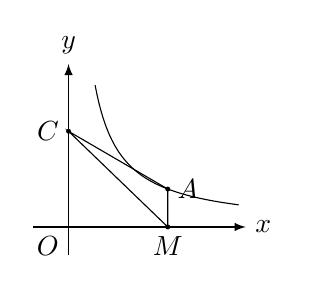
\begin{tikzpicture}[scale=0.45,>=latex]
  \draw[->] (-1,0)--(5,0) node[right]{$x$};
  \draw[->] (0,-0.8)--(0,4.6) node[above]{$y$};
  \node[below left] at (0,0){$O$};
  \draw[smooth,domain=0.75:4.8,samples=80] plot(\x,{3/\x});
  \coordinate (A) at (2.8,1.07);
  \coordinate (M) at (2.8,0);
  \coordinate (C) at (0,2.7);
  \draw (A)--(M)--(C)--cycle;
  \fill (A) circle(2pt) node[right]{$A$};
  \fill (M) circle(2pt) node[below]{$M$};
  \fill (C) circle(2pt) node[left]{$C$};
\end{tikzpicture}
\end{center}

  \answerarea[34mm]
  \setcounter{solstep}{0}
  \begin{solutionblock}
    \textbf{答案：}$k=18$\par\medskip
    \solstep{面积模型}{$AM=|y|$，点 $C$ 到 $AM$ 的距离为 $|x|$，所以 $S_{\triangle AMC}=\frac{|k|}{2}$。}
    \solstep{求 $k$}{$\frac{|k|}{2}=9$，得 $|k|=18$。图像在第一、三象限，所以 $k=18$。}
  \end{solutionblock}
\end{problem}


\needspace{8\baselineskip}

\begin{problem}[points=8]
  如图，点 $A$ 在反比例函数 $y=\dfrac{3-q}{x}$ 上，过 $A$ 向 $y$ 轴作垂线，垂足为 $N$。点 $D(-5,0)$ 在 $x$ 轴上。若 $\triangle AND$ 的面积为 $6$，且图像在第二、四象限，求 $q$。
\begin{center}
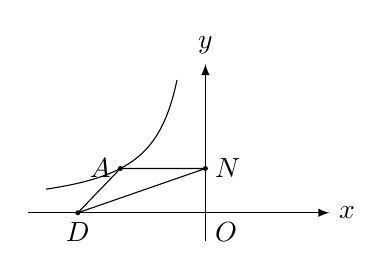
\begin{tikzpicture}[scale=0.45,>=latex]
  \draw[->] (-5,0)--(3.5,0) node[right]{$x$};
  \draw[->] (0,-0.8)--(0,4.2) node[above]{$y$};
  \node[below right] at (0,0){$O$};
  \draw[smooth,domain=-4.5:-0.8,samples=80] plot(\x,{-3/\x});
  \coordinate (A) at (-2.4,1.25);
  \coordinate (N) at (0,1.25);
  \coordinate (D) at (-3.6,0);
  \draw (A)--(N)--(D)--cycle;
  \fill (A) circle(2pt) node[left]{$A$};
  \fill (N) circle(2pt) node[right]{$N$};
  \fill (D) circle(2pt) node[below]{$D$};
\end{tikzpicture}
\end{center}

  \answerarea[36mm]
  \setcounter{solstep}{0}
  \begin{solutionblock}
    \textbf{答案：}$q=15$\par\medskip
    \solstep{面积模型}{$AN=|x|$，点 $D$ 到 $AN$ 的距离为 $|y|$，所以 $S_{\triangle AND}=\frac{|3-q|}{2}$。}
    \solstep{列方程}{$\frac{|3-q|}{2}=6$，所以 $|3-q|=12$。}
    \solstep{筛选}{图像在第二、四象限，所以 $3-q<0$，即 $3-q=-12$，得 $q=15$。}
  \end{solutionblock}
\end{problem}


\needspace{8\baselineskip}

\begin{problem}[points=8]
  如图，点 $A$ 在反比例函数 $y=\dfrac{k}{x}$ 当 $x<0$ 时的部分图像上。过点 $A$ 作 $AB\perp x$ 轴，交 $x$ 轴于点 $D$，且 $D$ 为线段 $AB$ 的中点；点 $C$ 为 $y$ 轴上一点。若 $\triangle ABC$ 的面积为 $9$，求 $k$。
\begin{center}
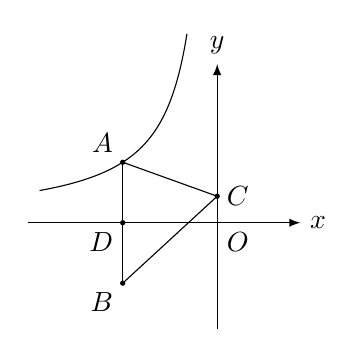
\begin{tikzpicture}[scale=0.48,>=latex]
  \draw[->] (-5,0)--(2.2,0) node[right]{$x$};
  \draw[->] (0,-2.8)--(0,4.2) node[above]{$y$};
  \node[below right] at (0,0){$O$};
  \draw[smooth,domain=-4.7:-0.8,samples=80] plot(\x,{-4/\x});
  \coordinate (A) at (-2.5,1.6);
  \coordinate (D) at (-2.5,0);
  \coordinate (B) at (-2.5,-1.6);
  \coordinate (C) at (0,0.7);
  \draw (A)--(B);
  \draw (A)--(C)--(B);
  \draw[dashed] (D)--(0,0);
  \fill (A) circle(2pt) node[above left]{$A$};
  \fill (B) circle(2pt) node[below left]{$B$};
  \fill (C) circle(2pt) node[right]{$C$};
  \fill (D) circle(2pt) node[below left]{$D$};
\end{tikzpicture}
\end{center}

  \answerarea[34mm]
  \setcounter{solstep}{0}
  \begin{solutionblock}
    \textbf{答案：}$k=-9$\par\medskip
    \solstep{设点坐标}{设 $A(x,y)$，则 $xy=k$。由图可知 $x<0,y>0$，所以 $k<0$。}
    \solstep{利用中点}{$D(x,0)$ 是 $AB$ 的中点，所以 $B(x,-y)$，从而 $AB=2|y|$。}
    \solstep{转化面积}{点 $C$ 在 $y$ 轴上，到直线 $AB$ 的距离为 $|x|$，所以 $S_{\triangle ABC}=\frac12\cdot2|y|\cdot|x|=|xy|=|k|$。}
    \solstep{确定符号}{$|k|=9$，且 $k<0$，故 $k=-9$。}
  \end{solutionblock}
\end{problem}


\needspace{8\baselineskip}

\begin{problem}[points=8]
  如图，点 $A$ 在反比例函数 $y=\dfrac{5-q}{x}$ 当 $x>0$ 时的部分图像上。过点 $A$ 作 $AB\perp x$ 轴，交 $x$ 轴于点 $D$，且 $D$ 为线段 $AB$ 的中点；点 $C$ 为 $y$ 轴上一点。若 $\triangle ABC$ 的面积为 $8$，求 $q$。
\begin{center}
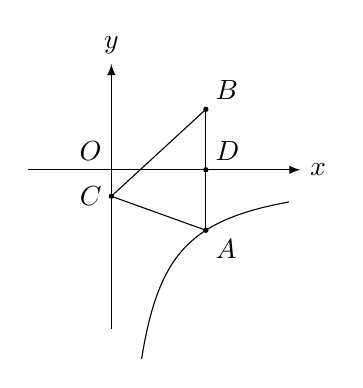
\begin{tikzpicture}[scale=0.48,>=latex]
  \draw[->] (-2.2,0)--(5,0) node[right]{$x$};
  \draw[->] (0,-4.2)--(0,2.8) node[above]{$y$};
  \node[above left] at (0,0){$O$};
  \draw[smooth,domain=0.8:4.7,samples=80] plot(\x,{-4/\x});
  \coordinate (A) at (2.5,-1.6);
  \coordinate (D) at (2.5,0);
  \coordinate (B) at (2.5,1.6);
  \coordinate (C) at (0,-0.7);
  \draw (A)--(B);
  \draw (A)--(C)--(B);
  \draw[dashed] (D)--(0,0);
  \fill (A) circle(2pt) node[below right]{$A$};
  \fill (B) circle(2pt) node[above right]{$B$};
  \fill (C) circle(2pt) node[left]{$C$};
  \fill (D) circle(2pt) node[above right]{$D$};
\end{tikzpicture}
\end{center}

  \answerarea[38mm]
  \setcounter{solstep}{0}
  \begin{solutionblock}
    \textbf{答案：}$q=13$\par\medskip
    \solstep{设点坐标}{设 $A(x,y)$，则 $xy=5-q$。由图可知 $x>0,y<0$，所以 $5-q<0$。}
    \solstep{利用中点}{$D(x,0)$ 是 $AB$ 的中点，所以 $B(x,-y)$，从而 $AB=2|y|$。}
    \solstep{转化面积}{点 $C$ 在 $y$ 轴上，到直线 $AB$ 的距离为 $|x|$，所以 $S_{\triangle ABC}=\frac12\cdot2|y|\cdot|x|=|xy|=|5-q|$。}
    \solstep{解参数}{$|5-q|=8$，且 $5-q<0$，所以 $5-q=-8$，得 $q=13$。}
  \end{solutionblock}
\end{problem}


\clearpage
\section*{答案速查}




\end{document}
